
\section{Modo Depuración}
La información respecto al movimiento de nuestros agentes la podemos consultar en el inspector en la parte derecha de unity siempre y cuando no ejecutemos el juego en pantalla completa. Para intentar hacer que algunos valores se consulten de forma más intuitiva se ha hecho uso de Gizmos y también de imágenes auxiliares.

Empezando por los Gizmos, estos son una clase especial de Unity que nos permite que sea activada y desactivada durante la ejecución a través del inspector como se ve en la figura \ref{fig:giz} y estos serán visibles en la escena.
\begin{figure}[H]
    \centering
    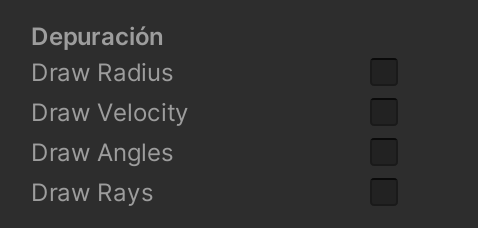
\includegraphics[scale=0.5]{doc/images/Gizmos.png}
    \caption{Gizmos disponibles}
    \label{fig:giz}
\end{figure}

Para que una clase pueda 'depurar' sus atributos será necesario que esta tenga un método llamado \textit{OnDrawGizmos}. Veamos por ejemplo el de la clase Agent que muestra los atributos de la figura anterior. 
\begin{lstlisting}
private void OnDrawGizmos()
	{
		if (drawAngles)
		{
			Gizmos.color = Color.red;
			Gizmos.DrawLine(Position,
				Position + OrientationToVector(Orientation + _interiorAngle) * DefaultLineLength);
			Gizmos.DrawLine(Position,
				Position + OrientationToVector(Orientation - _interiorAngle) * DefaultLineLength);
			
			Gizmos.color = Color.yellow;
			Gizmos.DrawLine(Position,
				Position + OrientationToVector(Orientation + _exteriorAngle) * DefaultLineLength);
			Gizmos.DrawLine(Position,
				Position + OrientationToVector(Orientation - _exteriorAngle) * DefaultLineLength);
		}
		if (drawVelocity)
		{
			Gizmos.color = Color.blue;
			Gizmos.DrawLine(Position, Position + Velocity);
		}

		if (drawRadius)
		{
			Gizmos.color = Color.magenta;
			Gizmos.DrawWireSphere(Position, _interiorRadius);
			
			Gizmos.color = Color.blue;
			Gizmos.DrawWireSphere(Position, _arrivalRadius);
		}

		if (drawRays && _rays != null)
		{
			Gizmos.color = Color.blue;
			foreach (Vector3 ray in _rays)
			{
				Gizmos.DrawLine(Position, Position + ray);
			}
		}
	}
\end{lstlisting}

En el bloque de código anterior podemos ver cómo se hace una comprobación por cada botón que aparece en la interfaz, y si ese gizmo está activado se procede a establecer el color del gizmo, la forma geométrica con la que lo queremos representar, ya sea una esfera o una linea en nuestro caso y este elemento geométrico tendrá como parámetros la posición en la que establecerse que suele ser la del Agente y el radio o la longitud según se quiera representar una velocidad, unos rayos de colisión o algún radio del Agente.\\

El otro elemento introducido a modo de depuración del comportamiento de los agentes, ha sido el de poder conocer el estado en el que está cada uno mediante el icono de estado que aparece a la izquierda del personaje. La implementación de este mecanismo ya se explicó en la sección \textbf{Interfaz gráfica y Jugabilidad}.